\section{Rotation af rigide legemer}


\begin{table}[ht]
\begin{tabular}{|l|l|l|}
\hline
\textbf{Givet}                                                                                             & \textbf{Ønsker at finde}   & \textbf{Relevante formler} \\ \hline
Ændring i vinkel, ændring i tid &
  Vinkelhastighed &
  \begin{tabular}[c]{@{}l@{}}\ref{afs:gnsvin} – Gennemsnitsvinkelhastighed\\ \ref{afs:insvin} – Øjebliksvinkelhastighed\end{tabular} \\ \hline
\begin{tabular}[c]{@{}l@{}}Ændring i vinkelhastighed, \\ ændring i tid\end{tabular} &
  Vinkelacceleration &
  \begin{tabular}[c]{@{}l@{}}\ref{afs:gnsvinacc} – Gennemsnitsvinkelacceleration\\ \ref{afs:insvinacc} – Øjebliksvinkelacceleration\end{tabular} \\ \hline
\begin{tabular}[c]{@{}l@{}}Initial vinkelhastighed, \\ vinkelacceleration, tid\end{tabular}                & Vinkelhastighed            & \ref{afs:vinhaskonvinacc}  \\ \hline
\begin{tabular}[c]{@{}l@{}}Initial- og slutvinkelhastighed, \\ tid, startvinkel\end{tabular}               & Vinkel                     & \ref{afs:vinkonvin}        \\ \hline
\begin{tabular}[c]{@{}l@{}}Initialvinkel, initialvinkelhas-\\ tighed, tid, vinkelacceleration\end{tabular} & Vinkel                     & \ref{afs:vinkonvinacc}     \\ \hline
\begin{tabular}[c]{@{}l@{}}Initialvinkelhastighed, vinkel-\\ acceleration, initial- og slutvinkel\end{tabular} &
  Vinkelhastighed &
  \ref{afs:vinhaskonvinaccvin} \\ \hline
Radius, vinkelhastighed                                                                                    & Tangential hastighed       & \ref{afs:tanhas}           \\ \hline
Radius, vinkelacceleration                                                                                 & Tangentiel acceleration    & \ref{afs:tanacc}           \\ \hline
Radius, vinkelhastighed                                                                                    & Radiel acceleration        & \ref{afs:cpacc}            \\ \hline
Masser, afstande                                                                                           & Inertimoment for et legeme & \ref{afs:inemomrot}        \\ \hline
Inertimoment, vinkelhastighed                                                                              & Rotationel kinetisk energi & \ref{afs:erotkin}          \\ \hline
Form                                                                                                       & Inertimoment               & \ref{afs:inemomforleg}     \\ \hline
\begin{tabular}[c]{@{}l@{}}Inertimoment, masse, afstand til\\  ny omdrejningsakse\end{tabular} &
  \begin{tabular}[c]{@{}l@{}}Inertimoment om ny\\ (parallel) omdrejningsakse\end{tabular} &
  \ref{afs:parakstheo} \\ \hline
\end{tabular}
\end{table}



\subsection{Vinkelhastighed og -acceleration (9.1)}

\subsubsection{Gennemsnitlig vinkelhastighed} \label{afs:gnsvin}
Analogt med \ref{afs:gnshas}: \nameref{afs:gnshas} kan den gennemsnitlige vinkelhastighed $\omega_{av-z}$, idet start- og slutvinklen i radianer $\theta_1$ og $\theta_2$ same start- og sluttidspunktet $t_1$ og $t_2$ er kendt, findes som
\[ 
\omega_{av-z} = \frac{\theta_2 - \theta_1}{t_2 - t_1} = \frac{\Delta \theta}{\Delta t}
.\]

\subsubsection{Øjebliksvinkelhastighed} \label{afs:insvin}
Analogt med \ref{afs:inshas}: \nameref{afs:inshas} kan øjebliksvinkelhastigheden $\omega_z$ findes som
\[ 
\omega_z = \lim_{\Delta t \to 0} \frac{\Delta \theta}{\Delta t} = \frac{\mathrm{d}\theta}{\mathrm{d}t} 
.\]
Hvor $\theta$ angiver vinklen i radianer og $t$ er tiden.


\subsubsection{Gennemsnitlig vinkelacceleration} \label{afs:gnsvinacc}
På samme måde som i \ref{afs:gnsvin}: \nameref{afs:gnsvin} kan den gennemsnitlige vinkelacceleration $\alpha_{av-z}$ findes som
\[ 
\alpha_{av-z} = \frac{\omega_{2z} - \omega_{1z}}{t_2 - t_1} = \frac{\Delta \omega_z}{\Delta t}
.\]
Hvor $\omega_{1z}$ og $\omega_{2z}$ er hhv. start- og slutvinkelaccelerationen og $t_1$ og $t_2$ er start- og sluttiden.


\subsubsection{Øjebliksvinkelacceleration} \label{afs:insvinacc}
På samme måde som i \ref{afs:insvin}: \nameref{afs:insvin} kan den øjeblikkelige vinkelacceleration $\alpha_{z}$ findes som
\[ 
\alpha_z = \lim_{\Delta t \to 0} \frac{\Delta \omega_z}{\Delta t} = \frac{\mathrm{d}\omega_{z}}{\mathrm{d}t} 
.\]
Hvor $\omega_z$ er vinkelaccelerationen og $t$ er tiden.


\subsection{Rotation med konstant vinkelacceleration (9.2)}

\subsubsection{Vinkelhastighed efter tid med konstant vinkelacceleration} \label{afs:vinhaskonvinacc}
Givet initialvinkelhastigheden $\omega_{0z}$, vinkelaccelerationen $\alpha_z$ samt tiden $t$ kan vinkelhastigheden $\omega_z$ til tiden $t$ findes som
\[ 
\omega_z = \omega_{0z} + \alpha_z t
.\]


\subsubsection{Ændring i vinkel efter tid med konstant vinkelacceleration givet start- og slutvinkelhastighed} \label{afs:vinkonvin}
Givet initial- og slutvinkelhastigheden hhv. $\omega_{0z}$ og $\omega_z$, tiden $t$ og initialvinklen $\theta_0$ kan vinklen $\theta$ til tiden $t$ findes som
\[ 
\theta = \frac{1}{2}(\omega_{0z} + \omega_z)t + \theta_0
.\]

\subsubsection{Ændring i vinkel efter tid med givet konstant vinkelacceleration} \label{afs:vinkonvinacc}
Givet startvinklen $\theta_0$, startvinkelhastigheden $\omega_{0z}$ og vinkelaccelerationen $\alpha_{z}$ kan vinklen $\theta$ til tiden $t$ findes som
\[ 
\theta = \theta_0 + \omega_{0z}t + \frac{1}{2}\alpha_z t^2
.\]

\subsubsection{Vinkelvastighed ved konstant vinkelacceleration givet start-vinkelhastighed, vinkelaccelerationen og start- og slutvinkel} \label{afs:vinhaskonvinaccvin}
Givet initialvinkelhastigheden $\omega_{0z}$, vinkelaccelerationen $\alpha_z$ og start- og slutvinklen hhv. $\theta_0$ og $\theta$ kan vinkelhastigheden $\omega_z$ findes som
\[ 
\omega_z = \sqrt{\omega_{0z}^2 + 2\alpha_z (\theta - \theta_0)}
.\]


\subsection{Sammenhæng mellem lineær og rotationskinematik (9.3)}

\subsubsection{Tangentiel hastighed for punkt på roterende objekt} \label{afs:tanhas}
Givet vinkelhastigheden $\omega$ af et roterende objekt og afstanden $r$ til rotationsaksen kan den tangentielle hastighed $v_{\text{tan}}$ for ethvert punkt på det roterende objekt findes som
\[ 
v_{\text{tan}} = r\omega
.\]

\subsubsection{Tangentiel acceleration for et roterende rigidt legeme} \label{afs:tanacc}
Den tangentielle acceleration $a_{\text{tan}}$ kan findes som
\[ 
a_{\text{tan}} = \frac{\mathrm{d}v}{\mathrm{d}t} = r \frac{\mathrm{d}\omega}{\mathrm{d}t} = r\alpha
.\]
Hvor $v$ er hastigheden, $r$ er afstanden til rotationsaksen, $\omega$ er vinkelhastigheden, $t$ er tiden og $\alpha$ er vinkelaccelerationen


\subsubsection{Centripetalacceleration} \label{afs:cpacc}
Centripetalaccelerationen til et givent punkt $a_{\text{rad}}$ kan findes som
\[ 
a_{\text{rad}} = \frac{v_{\text{tan}}^2}{r} = \omega^2 r
.\]
Hvor $v_{\text{tan}}$ er den tangentielle hastighed til det givne punkt, $r$ er afstanden fra det givne punkt til rotationsaksen og $\omega$ er vinkelhastigheden til det givne punkt.


\subsection{Energi for roterende bevægelse (9.4)}

\subsubsection{Inertimoment for et legeme om en given rotationsakse} \label{afs:inemomrot}
Inertimomentet $I$ for et legeme om en given rotationsakse kan findes som
\[ 
I = m_1 r_1^2 + m_2r_2^2 + \ldots  = \sum_i m_i r_i^2 = \int r^2 \, \mathrm{d}m
.\]
Hvor $m_1, m_2, \ldots $ er masserne af partiklerne der indgår i legemet og $r_1, r_2, \ldots$ er den vinkelrette afstand fra partiklerne til rotationsakserne.

\subsubsection{Rotationel kinetisk energi} \label{afs:erotkin}
Givet inertimomentet $I$ om en given omdrejningsakse og vinkelhastigheden $\omega$ om den givne omdrejningsakse kan den rotationelle kinetiske energi $K$ om selvsamme omdrejningsakse findes som
\[ 
K = \frac{1}{2} I \omega^2
.\]

\subsubsection{Inertimomenter for forskellige legemer} \label{afs:inemomforleg}
Følgende oversigt (\textbf{\autoref{fig:F1}}) over inertimomenter for forskellige legemer er hentet fra bogens side 285.
\begin{figure} [ht]
  \centering
  \caption{Inertimomenter for forskellige legemer}
  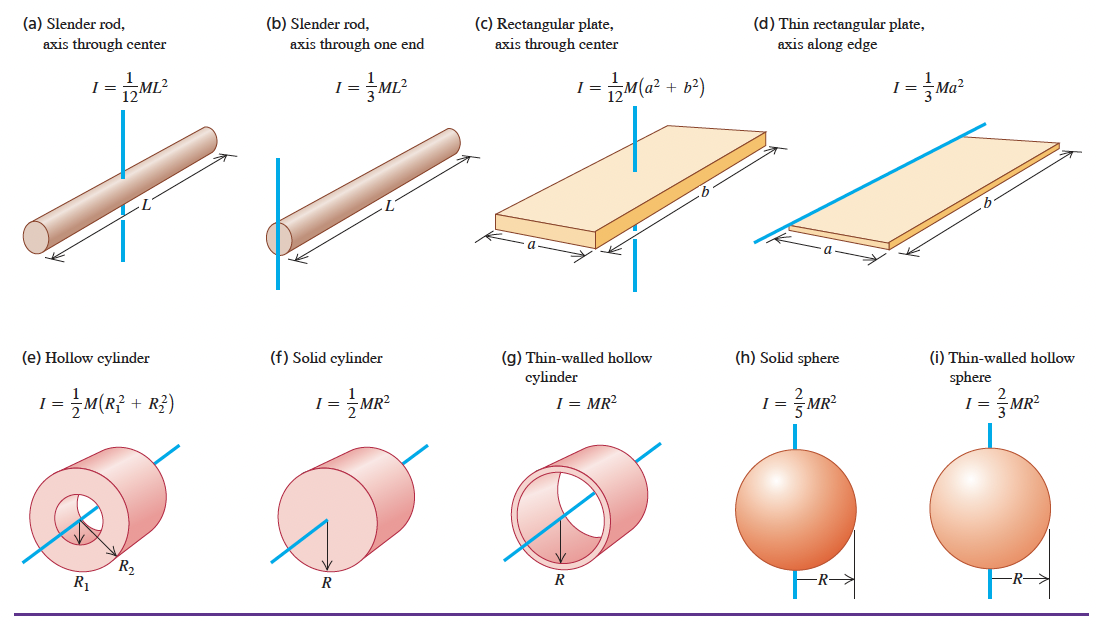
\includegraphics[width=0.8\linewidth]{../figures/F1.png}
  \label{fig:F1}
\end{figure}


\subsection{Parallel-akse-teoremet} \label{afs:parakstheo}
Parallel-akse-teoremet foreskriver at
\[ 
I_{P} = I_{\text{cm}} + Md^2
.\]
Hvor $M$ er massen af legemet, $I_{P}$ er inertimomentet for rotation gennem punktet $P$, $I_{\text{cm}}$ er inertimomentet for en akse gennem legemets massemidtpunkt, der er parallel med aksen gennem $P$ og $d$ er afstanden fra massemidtpunktet til punktet $P$.
